\documentclass[secnumarabic,nobalancelastpage,10pt,nofootinbib,a4paper]{memoir}
%\documentclass[aps,secnumarabic,nobalancelastpage,amsmath,amssymb,
%nofootinbib]{revtex4}

% secnumarabic is a particularly nice way of identifying sections by
% number to aid electronic review and commentary.


\usepackage[spanish, activeacute]{babel} %Definir idioma español
\usepackage[utf8]{inputenc} %Codificacion utf-8
\usepackage[T1]{fontenc}

\usepackage{graphics}      % standard graphics specifications
\usepackage{graphicx}      % alternative graphics specifications
\usepackage{url}           % for on-line citations
\usepackage{hyperref}
%\usepackage{cleveref}
\usepackage{bm}            % special 'bold-math' package

\usepackage{amsmath,amssymb,amsfonts}
\usepackage{physics}
\usepackage[exponent-product=\cdot,range-phrase=--,range-units=single]{siunitx}

\usepackage{longtable}     % helps with long table options
\usepackage{booktabs}
\usepackage{tabularx}
\usepackage{babelbib}
\usepackage{epigraph}

%\setlength{\paperheight}{11in}
\usepackage{todonotes}
\usepackage{microtype}

\graphicspath{{images/}}

\newcommand{\ra}[1]{\renewcommand{\arraystretch}{#1}}
\setlength{\parindent}{0pt}


\begin{document}

\listoftodos

\title{La temperatura de Hagedorn y la entropía de agujeros negros}
\author         {John Liu Anta
                \\ Universidad de Oviedo}
\date{\today}

\maketitle
\thispagestyle{empty}

\frontmatter

\tableofcontents*

\mainmatter

\renewcommand{\baselinestretch}{1.50}\normalsize

\chapter*{Resumen}

Este trabajo tiene como objetivo entender cómo la temperatura de Hagedorn, 
caractéristica de todas las teorías de cuerdas, se ve afectada por la presencia de agujeros
negros.

La base de este trabajo es la tesis \cite{Mertes2015}, en la cual se determina que la temperatura
de Hagedorn 
En el capítulo 1 se introducen los conceptos fundamentales de teoría de cuerdas.
En el capítulo 2, se analiza la termodinámica de una gas de cuerdas en
espacio de Minkowski, donde aparece la temperatura de Hagedorn.
El capítulo 3 trata dos aspectos de considerar una teoría cuántica de campos en 
sistemas de refencia no inerciales: la temperatura de Unruh y la temperatura de Hawking.
El concepto de partícula es dependiente del observador.
El estudio de cuerdas en espacios curvos se realiza en el capítulo 4. 



\ldots



\chapter{Introducción a la teoría de cuerdas}


\section{Motivación}

\todo{Describir brevemente objetivos, utilidad y estado actual}


\todo{Convenio}
Tomamos una métrica con signatura $(-+++)$.
\todo{Decir cuerda cerrada y bosonica}

\section{La cuerda relativista}

\todo{Métrica, linea de universo}

La teoría de cuerdas parte de considerar que las entidades fundamentales son cuerdas
en vez de partículas. 


La trayectoria $\mathbf x(t)$ de una partícula satisface que su acción $S$ es un extremal.
Coloquialmente, esto significa que la variación de la acción a primer orden es nula bajo
variaciones pequeñas de la trayectoria, supuestas fijas las posiciones iniciales y finales.
La acción de una partícula libre es
\begin{equation}
  S=-m\int dt \sqrt{1-\dot {\vec{x}} \cdot \dot {\vec{x}}},
\end{equation}
donde $\dot x = \dv{x}{t}$.

Para que en la acción aparezca el tiempo y la posición en igualdad de condiciones,
parametrizamos el tiempo y la posición por el tiempo propio $\tau$. 
El tiempo propio es el tiempo que mediría un reloj que se moviese con la partícula.
Con esta transformación, la acción es
\begin{equation}
 S = -m\int d\tau \sqrt{-\dv{x_\mu}{\tau}\dv{x^\mu}{\tau}}=-m\int d\tau .
\end{equation}


Generalizaremos la acción de una partícula libre a una cuerda libre.
Una cuerda está parametrizada por una variable temporal $\tau$ y una variable espacial $\sigma$, adimensional.
De forma más compacta, $(\sigma^0,\sigma^1)=(\tau,\sigma)$. 
La trayectoria de la cuerda en el espacio-tiempo genera un superficie llamada \emph{worldsheet}.
Las coordenadas en la worldsheet determinan un punto del espacio-tiempo $X^\mu$, también llamado
espacio \emph{target} para evitar confusión.

Para una cuerda cerrada con periodicidad $2\pi$, identificamos $X^\mu(\tau,\sigma)=X^\mu(\tau,\sigma+2\pi)$.

La acción de una partícula es proporcional a la longitud de su línea de universo.
De forma análoga, la acción de una cuerda debería ser proporcional al área de la
worldsheet.
Para poder medir el área, es necesario definir una métrica $\gamma_{\alpha\beta}$ en la worldsheet.
La forma natural de definir una métrica en una superficie, a partir de la métrica del espacio que
contiene a la superficie, es mediante el concepto de \emph{pull-back}.
En este caso, la métrica en la worldsheet el pull-back de la métrica de Minkowski
\begin{equation}
  \gamma_{ab}=\pdv{X^\mu}{\sigma^\alpha}\pdv{X^\nu}{\sigma^\beta}\eta_{\mu\nu}.
\end{equation}

La propiedad esencial de la métrica $\gamma_{\alpha\beta}$ es que la distancia entre dos puntos próximos 
coincide con la calcula con la métrica $\eta_{\mu\nu}$, ya que
\begin{equation}
  g_{\mu\nu}(X(\sigma)) dX^\mu(\sigma)dX^\nu(\sigma) = \gamma_{\alpha\beta} d\sigma^\alpha d\sigma^\beta.
\end{equation}



La medida de integración invariante bajo cambios generales de coordenadas más sencilla 
es $d^2\sigma \sqrt{-\det\gamma}$, por lo que la acción, llamada de Nambu-Goto, es
\begin{equation}
  S_{NG}=-T\int d^2\sigma \sqrt{-\det\gamma}.
\end{equation}

El parámetro $T$ se corresponde con la tensión de la cuerda y se puede expresar como
\begin{equation}
  T=\frac{1}{2\pi\alpha'},
\end{equation}
donde $\alpha'$ es la pendiente de Regge.

A la hora de cuantizar la teoría, la raíz cuadrada es problemática, por lo que se introduce
un campo tensorial $h$ definido sobre la worldsheet en la llamada acción de Polyakov
\begin{equation}
  S_P=-\frac{1}{4\pi\alpha'}\int d^2\sigma  \sqrt{-h}h^{\alpha\beta}\partial_\alpha X^\mu \partial_\beta X_\mu.
\end{equation}

Este campo $h$ se comporta como una métrica en dos dimensiones y queda fijada por las
ecuaciones de movimiento
\begin{equation}
  h_{\alpha\beta}=2f(\sigma)\partial_\alpha X^\mu \partial_\beta X_\mu
\end{equation}
donde $f(\sigma)$ es una función cualquiera. La libertad de poder escoger $f(\sigma)$
es una simetría gauge

\todo{Simetría gauge, Weyl}


\section{Cuantización}

Debido a la simetría gauge de la teoría, la cuantización no es directa.
Hay grados de libertad que no son físicos y en algún momento hemos de deshacernos de ellos.
Para obtener directamente una teoría unitaria, cuantizamos solo los grados de libertad 
físicos, buscando primero las soluciones clásicas. 
Como contrapartida, perdemos la invariancia de Lorentz explícita.

Definimos las coordenadas en el cono de luz
\begin{equation}
  \sigma^\pm=\tau\pm\sigma
\end{equation}

y
\begin{equation}
  X^\pm=\frac{1}{\sqrt 2} (X^0 \pm X^{d-1}).
\end{equation}

Gracias a la simetría gauge, imponemos $h_{\alpha\beta}=\eta_{\alpha\beta}$, de forma que 
la acción de Polyakov es
\begin{equation}
  S = -\frac{1}{4\pi\alpha'} \int d^2\sigma \partial_\alpha X^\mu \partial^\alpha X_\mu,
\end{equation}
que da lugar a la ecuaciones de movimiento de ondas libres
\begin{equation}
  \partial_\alpha \partial^\alpha X^\mu=0.
\end{equation}

La solución general de la ecuación de movimiento para $X^+$ se descompone
en una onda moviéndose hacia la izquierda $X^+_L$ y otra hacia la derecha $X^+_R$,
\begin{equation}
   X^+ =X^+_L(\sigma^+) + X^+_R(\sigma^-).
\end{equation}

Teniendo en cuenta la periodicidad en $\sigma$, la expansión de Fourier conduce a
\begin{equation}
  \begin{gathered}
    X^+_L=\frac 1 2 x^+ + \frac 1 2 \alpha' p^+ \sigma^+ + i\sqrt{\frac{\alpha'}{2}}\sum_{n\neq 0} \frac{1}{n}\tilde \alpha^+_n e^{-in\sigma^+},\\
    X^+_R=\frac 1 2 x^+ + \frac 1 2 \alpha' p^+ \sigma^- +i\sqrt{\frac{\alpha'}{2}}\sum_{n\neq 0} \frac{1}{n}\alpha^+_n e^{-in\sigma^-}.
  \end{gathered}
\end{equation}
Donde $x^+$ y $p^+$ se corresponden con la posición y el momento del centro de masas, respectivamente.


Debido a la invariancia baja reparametrizaciones, escogemos
\begin{equation}
  X^+_L=\frac 1 2 x^+ + \frac 1 2 \alpha' p^+ \sigma^+,
\end{equation}
y
\begin{equation}
  X^+_R=\frac 1 2 x^+ + \frac 1 2 \alpha' p^+ \sigma^+.
\end{equation}

Por tanto, 
\begin{equation}
  X^+ = x^+ + \alpha' p^+ \tau.
\end{equation}
La constante $x^+$ puede eliminarse mediante una traslación en $\tau$.

Con esta elección gauge, la solución $X^-$ que determinada casi por completo.
La ecuación de movimiento para la métrica $h$ se obtiene variando a acción
\begin{equation}
  \delta S = \frac{1}{4\pi\alpha'}\int d^2\sigma \delta h^{\alpha\beta}
  \qty(
  \sqrt{-h}\partial_\alpha X^\mu \partial_\beta X_\mu -
  \frac 1 2 \sqrt{-h}h_{\alpha\beta}h^{\rho\sigma} \partial_\rho X^\mu \partial_\sigma X_\mu).
\end{equation}
Como habíamos elegido $h_{\alpha\beta}=\eta_{\mu\nu}$, la ecuación de movimiento impone
\begin{equation}
  \partial_\alpha X^\mu \partial_\beta X_\mu - \frac 1 2 \eta_{\alpha\beta} \eta^{\sigma\rho} 
  \partial_\rho X^\mu  \partial_\sigma X_\mu = 0.
\end{equation}

En las coordenadas del cono de luz, esto se traduce en
\begin{equation}
  (\partial_+ X)^2 = (\partial_- X)^2 = 0.
  \label{eq:lig}
\end{equation}

Haciendo la descomposición de la solución $X^-$ 
\begin{equation}
  X^-=X^-_L(\sigma^+)+X^-_R(\sigma^-),
\end{equation}
la ecuación \ref{eq:lig} conduce a 
  \begin{align}
    \partial_+ X_L^- = \frac{1}{\alpha'p^+}\sum_{i=1}^{d-2} \partial_+ X^i \partial_+ X^i, \label{eq:lig1}\\
    \partial_- X_R^- = \frac{1}{\alpha'p^-}\sum_{i=1}^{d-2} \partial_- X^i \partial_- X^i. \label{eq:lig2}
  \end{align}

En el desarrollo de Fourier
\begin{equation}
  \begin{gathered}
    X^-_L(\sigma^+)=\frac 1 2 x^- + \frac 1 2 \alpha' p^- \sigma^+ + i\sqrt{\frac{ \alpha'}{ 2}}
    \sum_{n\neq0} \frac 1 n \tilde{\alpha}^-_n e^{-in\sigma^+} \\                             
    X^-_R(\sigma^+)=\frac 1 2 x^- + \frac 1 2 \alpha' p^- \sigma^- + i\sqrt{\frac{ \alpha'}{ 2}}
    \sum_{n\neq0} \frac 1 n \alpha^-_n e^{-in\sigma^-},
  \end{gathered}
\end{equation}
las constantes $p^-$, $\tilde \alpha^-_n$ y $\alpha^-_n$ quedan determinadas por las ecuaciones
\ref{eq:lig1} y \ref{eq:lig2}.

El momento $p^-$ se puede expresar a través de $\alpha^i_n$ y de $\tilde \alpha^i_n$ como
\begin{equation}
  p^- = \frac{1}{\alpha' p^+}\sum_{i=1}^{d-2} \qty(\frac{1}{2}\alpha'p^i p^i +\sum_{n\neq0}\alpha_n^i\alpha_{-n}^i) 
   = \frac{1}{\alpha' p^+}\sum_{i=1}^{d-2} \qty(\frac{1}{2}\alpha'p^i p^i +\sum_{n\neq0}\tilde \alpha_n^i\tilde \alpha_{-n}^i) .
\end{equation}

La masa de la cuerda es por tanto
\begin{equation}
  M^2=-p_\mu p^\mu = 2p^+p^- - \sum_{i=1}^{d-2} p^i p^i = 
  \frac{2}{\alpha'}\sum_{i=1}^{d-2} \sum_{n\neq 0} \alpha_{-n}^i \alpha_n^i
  =\frac{2}{\alpha'}\sum_{i=1}^{d-2} \sum_{n\neq 0}\tilde \alpha_{-n}^i \tilde\alpha_n^i.
  \label{eq:mass}
\end{equation}

Hemos obtenido la solución clásica mediante los $2(d-2)$ modos de oscilación transversos 
$\alpha^i_n$ y $\tilde \alpha_n^i$ y las constantes $x^i$, $p^i$,$p^+$ y $x^-$, donde $i=1,\cdots d-2$.
La cuantización consiste en promover los grados de libertad a operadores (denotados
por un acento circunflejo) que satisfacen una reglas de conmutación.
\footnote{En realidad, debido a la simetría gauge, la cuantización se haría a partir de los
corchetes de Poisson de la teoría clásica. No tendremos en cuenta esta sutileza porque el
resultado es el mismo.}
Estas reglas son
\begin{equation}
  \begin{gathered}
    \qty[\widehat x^i,\widehat p^j] = i\delta^{ij}\qquad , \qquad [\widehat x^-,\widehat p^+] = -i,\\
    \qty[\widehat \alpha_n^i,\widehat \alpha_m^j]= \qty[\widehat {\tilde \alpha}_n^i,\widehat {\tilde \alpha}_m^j]= n \delta^{ij}\delta_{n+m,0}
  \end{gathered}
\end{equation}

Los estados físicos sobre los que actúan los operadores se construyen a partir de un estado 
de vacío $\ket{0;p}$, que describe una cuerda de momento $p$ en el estado fundamental.
El vacío verifica
\begin{equation}
  \widehat p^\mu \ket{0;p} = p^\mu \ket{0;p} \qquad, \qquad \widehat \alpha^i_n\ket{0;p}=\widehat {\tilde\alpha}^i_n = 0 \qquad \text{con} \quad n>0.
\end{equation}

Las distintas excitaciones de la cuerda se obtienen aplicando $\alpha_{-n}^i$ y $\widehat{\tilde\alpha}_{-n}^i$
con $n>0$ sobre el vacío.
Cada excitación de la cuerda corresponde a una partícula, como veremos más adelante.

La fórmula de masas es análoga al caso clásico \ref{eq:mass} salvo una diferencia importante.
Clásicamente el producto de $\alpha^i_{-n}$ y $\alpha^i_n$ conmuta, por lo que hay una 
ambigüedad en el orden a asignar a los operadores $\widehat\alpha^i_{-n}$ y $\widehat \alpha^i_n$.
La ambigüedad introduce una constante $c$ desconocida en el operador de la masa al cuadrado,
\begin{equation}
  \widehat M^2 = \frac{4}{\alpha'}\qty(\sum_{i=1}^{d-2} \sum_{n>0} \alpha_{-n}^i\alpha_n -c)
   = \frac{4}{\alpha'}\qty(\sum_{i=1}^{d-2} \sum_{n>0} \tilde \alpha_{-n}^i\tilde \alpha_n -c).
\end{equation}

Por conveniencia, definimos los operadores número
\begin{equation}
  \widehat N=\sum_{i=1}^{d-2} \sum_{n>0}\widehat \alpha_{-n}^i\widehat\alpha_n^i \quad , \quad   
  \widehat {\tilde N}=\sum_{i=1}^{d-2} \sum_{n>0} \widehat{\tilde \alpha}_n^i\widehat{ \tilde\alpha}_n^i, 
\end{equation}
por lo que 
\begin{equation}
  \widehat M^2 = \frac{4}{\alpha'} (\widehat N -c ) = \frac{4}{\alpha'} (\widehat{\tilde N} -c).
\end{equation}

La condición $\widehat N=\widehat {\tilde N}$ se conoce como \emph{level-matching}.

La forma general de determinar $c$ (la carga central) consiste en imponer la simetría Weyl.
Nosotros no entraremos en los detalles, nos basta saber que para cuerdas bosónicas libres
bosónicas, $c=\frac{d-2}{24}$.


\subsection{Espectro de una cuerda}
En el estado de vacío, $\widehat N\ket{0;p}=\widehat {\tilde N}\ket{0;p}=0$, por lo que la masa es
\begin{equation}
  M^2 = -\frac{1}{\alpha'}\frac{d-2}{6}.
\end{equation}

Si $d>2$ la masa al cuadrado de la cuerda es negativa y la partícula a la que corresponde se denomina taquión.
Los taquiones aparecen también en teoría cuántica de campos al estudiar un campo $\phi$ con un 
potencial $V(\phi)$.
La masa de la partícula asociada al campo es
\begin{equation}
  M^2 = \pdv[2]{V(\phi)}{\phi}.
\end{equation}
Por tanto, una masa al cuadrado negativa indica que estamos haciendo una expansión en torno
a un máximo. 
Un ejemplo es el campo de Higgs cuando el valor del campo es cero.
A pesar de los problemas que introduce un taquión, no lo tendremos más en cuenta. 
De todas formas, al considerar cuerdas fermiónicas en la teoría supersimétrica, el taquión
desaparece.

El primer estado excitado se obtiene como
\begin{equation}
  \widehat{\tilde\alpha}_{-1}^i\widehat \alpha_{-1}^j\ket{0;p},
\end{equation}
con masa
\begin{equation}
  M^2 = \frac{4}{\alpha'}\qty(1-\frac{d-2}{24}).
\end{equation}

Teniendo en cuenta los valores posibles de $i$ y $j$ hay $(d-2)^2$ estados excitados.

\todo{Rematar}

Para que estos estados puedan describirse mediante la clasificación de Wigner de las
representaciones del grupo de Poincaré, los estados han de ser una representación $SO(d-2)$.
Esto significa que las partículas tienen masa nula, en caso contrario, se rompería la simetría
de Lorentz. Como $M^2=0$, obtenemos que la dimensión del espacio-tiempo es
\begin{equation}
  d=26.
\end{equation}
Además, la representación de estos estados se descompone un una parte simétrica, una antisimétrica
y una traza. Los campos asociados son el campo del gravitón $G_{\mu\nu}$, el campo Kalb-Ramond $B_{\mu\nu}$
y el dilatón $\Phi$, respectivamente.

Por tanto, la teoría bosónica predice métrica de la relatividad general $G_{\mu\nu}$ de forma 
natural, además de otro campo tensorial y un campo escalar.

Las siguientes excitaciones empiezan a tener masas del orden de la masa de Planck
\begin{equation}
  M_p=
\end{equation}
y están muy lejos de ser observadas. Sin embargo, el resto del trabajo se centrará en cuerdas
a esta escala de energía.


\subsection{Cuerdas supersimétricas}

La cuerdas supersimétricas describen tanto bosones como fermiones.
La teoría es supersimétrica porque a cada bosón le corresponde un fermión y vice versa.

Existen dos formas de incorporar fermiones:
en las cuerdas de tipo II, los fermiones se mueven en la worldsheet hacia la izquierda y a la derecha,
mientras que las cuerdas heteróticas, solo se mueven hacia la izquierda.
En ambos casos, la dimensión del espacio-tiempo es $d=10$.

\todo{Acabar}

\subsection{La integral de camino}

Una forma alternativa de cuantizar una teoría clásica consiste en la integral de camino, 
introducidad por Feynman. 
Sin entrar en detalles, la amplitud de probabilidad de que una partícula que está localizada 
en $(x_0,t_0)$, se detecte en $(x',t')$ se calcula teniendo en cuenta todas las trayectorias
que podría tomar la partícula entre estos dos puntos.
La amplitud de probabilidad asociada a cada trayectoria $x$ depende de la acción de esa trayectoria
como $e^{i/\hbar S[x]}$ y la amplitud total es simplemente la suma de las amplitudes de probabilidad
de todas las trayectorias posibles.
Las amplitudes de probabilidad difiere solo en la fase y no en la amplitud, por lo que habrá 
interferencia entre las distintas trayectorias.
En el límite clásico, la única contribución viene dada por la trayectoria clásica.

Formalmente, la amplitud de probabilidad se expresa mediante el propagador
\begin{equation}
  K(x',t';x_0,t_0) = \int \mathcal Dx e^{\frac{i}{\hbar} S[x]}.
\end{equation}

La integral no es integral el sentido habitual (Riemann o Lebesgue) y su definición matemática
es muy elaborada, pero basta tomarla en el sentido de suma de caminos.
Para evitar tratar con un integrando complejo, reemplazaremos el tiempo $t$ en la acción por un tiempo imaginario de modo que
\begin{equation}
  K(x',t';x_0,t_0) = \int \mathcal Dx e^{\frac{-1}{\hbar} S[x]}.
\end{equation}
Este procedimiento se conoce como rotación de Wick y su justificación matemática también presenta complicaciones.


La integral de camino en teoría de cuerdas se define de manera análoga, pero integramos 
sobre todas las trayectorias de la cuerda y sobre todas la métrica de la wordsheet,
\begin{equation}
  Z = \int \mathcal DX \mathcal Dh e^{-S_p+\lambda \chi}.
\end{equation}

En el exponente aparece un factor adicional $\lambda\chi$ que determina cómo contribuyen las trayectorias
de cuerdas con una determinada topología de la wordsheet.
La constante $\lambda$ determina cómo interaccionan las cuerdas entre sí y $\chi$ es la característica
de Euler de la wordlsheet.
La característica de Euler de una superficie de género $g$ (número de agujeros) es
\begin{equation}
  \chi = 2(1-g).
\end{equation}

\todo{Añadir dibujo}

Para incorporar interacciones de cuerdas con campos de fondo, introducimos términos adicionales a la acción.
Por ejemplo, el model sigma no lineal describe cuerdas propagándose en campos $G_{\mu\nu}$, $B_{\mu\nu}$ y $\Phi$.
\begin{equation}
  S = -\frac{1}{4\pi \alpha'}\int d^2 \sigma \sqrt h \qty[\qty(h^{\alpha\beta}G_{\mu\nu} + i\epsilon^{\alpha\beta}B_\mu\nu)\partial_\alpha X^\mu
  \partial_\beta X^\nu +\alpha'R\Phi].
\end{equation}

\subsection{Dualidad T}

Una propiedad muy importante de las teorías de cuerdas es la dualidad T.
Si consideramos cuerdas bosónicas con una dimensión espacial

\begin{equation}
  p_L = \frac{n}{R} + \frac{wR}{\alpha'} \qquad,\qquad  p_L = \frac{n}{R} - \frac{mR}{\alpha'} .
\end{equation}

La fórmula de masas es
\begin{equation}
  M^2 = \frac{n^2}{R^2} + \frac{w^2 R^2}{\alpha'^2} +\frac{2}{\alpha'}\qty(N+\tilde N -2).
\end{equation}

La transformación $R\to \alpha'/R$ $n\to w$


En presencia de campos adicionales, las reglas de transformación son
\begin{equation}
  \begin{gathered}
    G_{00}\to \frac{1}{G_{00}}, \quad G_{0i} \\
  \end{gathered}
\end{equation}





Definiendo
\begin{equation}
  L_n=\frac 1 2 \sum_m \alpha_{n-m} \cdot \alpha_m
\end{equation}

\begin{equation}
  \tilde{L}_n=\frac 1 2 \sum_m \tilde{\alpha}_{n-m} \cdot \tilde{\alpha}_m.
\end{equation}

Es importante ver que hay una expresión en términos de modos moviéndose a la derecha
y otra con modos moviéndose a la izquierda.



\chapter{Termodinámica de cuerdas}

\section{Cálculo de la densidad de estados para una cuerda excitada}

La fórmula de masas para una cuerda abierta es
\begin{equation}
  \alpha' m^2=-1+N
\end{equation}
y para una cuerda cerrada
\begin{equation}
  \alpha' m^2=-4+2(N+\bar N).
\end{equation}

\todo{Obtención de la densidad de estados en el paso al continuo}
Queremos calcular la densidad de estados de una cuerda en función del número de 
oscilador, 
\begin{equation}
  p(N)\approx \alpha N^ {\frac{d-1}{2}}\exp{\qty(2\pi\sqrt{\frac{N(d-2)}{6})}}.
\end{equation}

Expresando la densidad de estados en función de la masa
\begin{equation}
  p(M)\approx \alpha N^ {\frac{d-1}{2}}\exp{\qty(2\pi\sqrt{\frac{N(d-2)}{6})}}.
\end{equation}

\section{Modelo random walk}

\todo{Revisar planteamiento}
Intuitivamente, la masa (energía) de una cuerda es su densidad lineal $\sigma$ por su longitud $L$.
En unidades naturales, la masa tiene unidades inversas a la longitud, por lo que si pensamos
que la cuerda está dividida en $N$ segmentos de longitud $l_s$, 
\begin{equation}
  E\sim  \frac{N}{l_s} \sim \frac{L}{l_s^2}.
\end{equation}

Cada segmento podrá tener una orientación arbitraria. Para simplificar los cálculos,
supongamos que toma direcciones ortogonales. Entonces el número de orientaciones posibles
de cada segmento es $2n$, donde $n$ es el número de dimensiones espaciales accesibles.
El número de segmentos es $L/l_s$.
Por tanto, el número de microestados para una energía dada es
\begin{equation}
  \omega(E)=(2n)^{(L/l_s)}\propto e^{l_s E \ln (n)}.
\end{equation}

La entropía de la cuerda es $S\propto El_s$, con temperatura $\beta_H\sim l_S$.

Se puede calcular que el radio del random walk es $R=\expval{r}\sim E^{1/2}$. Esto
nos dice que cuerdas muy largas estarán contenidas en un volumen pequeño $V\sim E^{D/2}$.

Para una cuerda cerrada, habría que dividir el número de microestados por el 
volumen de walk, multiplicar por el volumen accesible y dividir por la longitud de la cuerda.
Entonces,
\begin{equation}
  \omega(E)\sim V \frac{e^{\beta_H E}}{E^{1+D/2}}.
\end{equation}

\todo{No necesitamos conocer los detalles de la teoría}
De esta forma, obtenemos la densidad de estados 

El cálculo de la extensión de una cuerda altamente excitada con respecto a su centro de masas 
conduce a que $R^2_i$ es proporcional a la suma de las inversas de los números oscilatorios para
la dirección $i$.
Por ello, para un nivel energético $N$ fijo, $(\alpha^i_{-1})^N\ket{0}$ tendría la mayor extensión en la dirección $i$, $\sim N$ y
$\alpha^i_N\ket{0}$ tendría la menor extensión.
Tomando el promedio sobre todas las direcciones espaciales, $R^2\sim (d-1)\sqrt{N}$, siendo
$d-1$ el número de direcciones espaciales. Volvemos a  observa la importante peculariadad $R\sim \sqrt{L}$,
por lo que las cuerdas largas tiende a enmarañarse.

\section{Coalescencia multicuerda}

\todo{Repaso de las colectividades estadísticas}

\subsection{Formulación microcanónica}


\subsection{Formulación canónica}

\section{Termodinámica de cuerdas en espacio plano}

%Termodinámica de cuerdas. Energía libre. Invariancia modular explícita. Escalar termal.

La función de partición bosónica en un espectro discreto es $z=\prod_i 1/(1-\exp(-\beta E_i))$.
La energía libre viene dada por $F=-1/\beta \ln z=\beta\sum_i \ln(1-\exp(-\beta E_i))$.
En el caso continuo, donde $E=E(k)$, reemplazamos el sumatorio por $V\int d^{d-1}k/(2\pi)^{d-1}$.
Por tanto,
\begin{equation}
  F=\frac{V}{\beta}\int \frac{d^{d-1}k}{(2\pi)^{d-1}}\ln(1-\exp(-\beta E))
\end{equation}

Mediante el desarrollo de Taylor $\ln(1-x)=-\sum^\infty_{r=1} x^r/r$
\begin{equation}
  F=-\frac{V}{\beta}\sum^\infty_{r=1} \frac 1 r\int \frac{d^{d-1}k}{(2\pi)^{d-1}}\exp(-r\beta E)
\end{equation}

Aplicando la identidad
\begin{equation}
  \frac 1 r \exp(-\beta r E)=\frac{\beta}{\sqrt{2\pi}}\int_0^\infty \frac{ds}{s^{3/2}}\exp\qty(-\frac{E^2s}{2}-\frac{r^2\beta^2}{2s})
\end{equation}

y como $E^2=k^2+m^2$

\begin{equation}
  F=-\frac{V}{\sqrt{2\pi}}\sum^\infty_{r=1} \int_0^\infty \frac{ds}{s^{3/2}} \exp \qty(-\frac{m^2s}{2} -\frac{r^2\beta^2}{2s})
  \int \frac{d^{d-1}k}{(2\pi)^{d-1}}\exp\qty(-\frac{k^2s}{2})
\end{equation}

La última integral tiene como resultado $(2\pi s)^{\frac{d-1}{2}}$, por lo que
\begin{equation}
  F=-V \int_0^\infty \frac{ds}{s(2\pi s)^{d/2}}\sum^\infty_{r=1} \exp \qty(-\frac{m^2s}{2}- \frac{r^2\beta^2}{2s})
\end{equation}

Por otro lado, la función de partición de estado multicuerda es $Z=e^z=-\beta F$. 
Entonces podemos hacer la asociación de la energía libre con integral de camino de 
una partícula tras aplicar una rotación de Wick en la dimensión temporal y compactificando el
tiempo con periodo $\beta$
\begin{equation}
  Z=-\beta F= \int_0^\infty \frac{ds}{2s}\sum^{'\infty}_{w=-\infty} \int \mathcal{D}x 
  \exp\qty(-\frac 1 2 \int_0^s d\tau \qty[\qty(\pdv{X^\mu}{t})^2+m^2])
\end{equation}

Se llega al mismo resultado calculando la función de partición de una partícula  si identificamos 
el parámetro $s$ con el tiempo propio  de la partícula y compactificamos 
la coordenada $X^0$ con periodo $\beta$. El número de vueltas que da la
partícula en la dimensión temporal es $w$. La función de partición se suma sobre
todas las vueltas posibles y se integra en todos los tiempos propios.

En una teoría de cuerdas bosónica, $d=26$ y la energía libre se obtendría sumando las
energías libres para todo el espectro posible, con masas
\begin{equation}
  m^2=\frac{2}{\alpha'}(N+\bar N-2)
\end{equation}

Puesto que se tiene que cumplir el level-matching $N=\bar N$, habrá que incluir en la 
integral la expresión de la delta de Kronecker
\begin{equation}
   \delta_{N\bar N}=\int_{-1/2}^{1/2}d\tau_1 \exp(2\pi i\tau_1 (N-\bar N))
\end{equation}

Entonces
\begin{equation}
  F=\sum_i \delta_{N_i \bar N_i} F(N_i,\bar N_i)
\end{equation}

donde $i$ recorre todas las posibles combinaciones de $N_i$ y $\bar N_i$.
Haciendo el cambio de variable $s=2\pi\alpha'\tau_2$
\begin{equation}
  F=-V \int_0^\infty \frac{d\tau_2}{\tau_2(4\pi^2\alpha'\tau_2)^{d/2}}\frac 1 2\sum_{r=-\infty}^{'\infty} 
  \sum_i e^{-(N_i+\bar N_i -2)2\pi\tau_2} e^{-\frac{r^2\beta^2}{4\pi\alpha'\tau_2}}\int_{-1/2}^{1/2} d\tau_1 e^{2\pi i\tau_1(N_i-\bar N_i)}
\end{equation}

Definiendo $\tau=\tau_1+i\tau_2$ y $q=e^{2\pi i\tau_1}$, se introduce la $\eta$ de 
Dedekind como
\begin{equation}
  \eta(\tau)=q^{1/24}\prod_{n=1}^{\infty} (1-q^n)
\end{equation}

Se llega a
\begin{equation}
  F=-V \sum_{r=-\infty}^{'\infty} \int_0^\infty\frac{d\tau_2}{2\tau_2} \int_{-1/2}^{1/2} d\tau_1  \frac{1}{(4\pi^2\alpha'\tau_2)^{d/2}}
  \abs{\eta(\tau)}^{-2d+4}\exp\qty(-\frac{r^2\beta^2}{4\pi\alpha'\tau_2})
\end{equation}

El mismo resultado se obtiene calculando la integral de camino en el toro
\begin{equation}
  Z= \int_0^\infty\frac{d\tau_2}{2\tau_2} \int_{-1/2}^{1/2} d\tau_1 \Delta_{FP} \int \mathcal Dx
  \exp\qty(-\frac{1}{4\pi\alpha'}\int d^2\sigma \sqrt h h^{\alpha\beta}\partial_\alpha X^\mu \partial_\beta X_\mu)
\end{equation}

donde la región de 

Se ha llegado a una expresión cuyo integrando no es modular invariante. Es decir, 
$\tau\to\tau+1$ y $\tau\to1/\tau$ no son invariancias.
Para conseguir la invariancia modular se restringe el dominio de integración al dominio
fundamental y se modifica el integrado, añadiendo el número cuántico $w$ sobre el que 
se suma, de modo que para $d=26$ se tiene
\begin{equation}
  F=-V \sum_{r,w=-\infty}^{\infty} \int_\mathcal{F}  \frac{d\tau_1d\tau_2}{2\tau_2}   \frac{1}{(4\pi^2\alpha'\tau_2)^{13}}
  \abs{\eta(\tau)}^{-48}\exp\qty(-\frac{\abs{r^2-w\tau}^2\beta^2}{4\pi\alpha'\tau_2})
\end{equation}

Haciendo la suma, se llega a
\begin{equation}
  Z=-\beta F=\int_{\mathcal F}\frac{d\tau_1d\tau_2}{2\tau_2}\Tr\qty(q^{L_0}\bar q^{\bar L_0})
\end{equation}

donde
\begin{align}
  L_0&=\alpha'\frac{p^2}{4}+\frac{\alpha'}{4}\qty(\frac{2\pi n}{\beta}+\frac{w\beta}{2\pi\alpha'})^2+N\\ 
 \bar L_0&=\alpha'\frac{p^2}{4}+\frac{\alpha'}{4}\qty(\frac{2\pi n}{\beta}-\frac{w\beta}{2\pi\alpha'})^2+\bar N
\end{align}


%\section{Cuerdas en background estático}
%Supongamos una cuerda en presencia de un background $G_{\mu\nu}$ independiente del tiempo.
%La función de partición calculada como la integral de camino en el toro es
%\begin{equation}
%  Z= \int_0^\infty\frac{d\tau_2}{2\tau_2} \int_{-1/2}^{1/2} d\tau_1 \Delta_{FP} \int \mathcal Dx \sqrt G
%  \exp\qty(-\frac{1}{4\pi\alpha'}\int d^2\sigma \sqrt h h^{\alpha\beta}\partial_\alpha X^\mu \partial_\beta X^\nu G_{\mu\nu})
%\end{equation}
%
%La métrica de la worldsheet

\section{Discrepancia entre colectividad microcanónica y canónica}

\todo{Comentar más allá de Hagedorn?}


\chapter{QFT en sistemas acelerados y espacio curvo}
%\todo{Corregir numeracion}

%\todo{Mejor meter subsecciones?}
\section{Efecto Unruh}

Una propiedad sorprendente de las teorías cuánticas de campos es que el estado de vacío
puede depender del observador.
Concretamente, el efecto Unruh establece que el vacío para un observador inercial,
visto por un observador con aceleración constante corresponde con un estado térmico a temperatura
\begin{equation}
  T_U=\frac{a}{2\pi k_B}.
\end{equation}
En este apartado, seguiremos la derivación expuesta en \cite{Barbado:2015uua}.

En la deducción del efecto Unruh estudiaremos un campo escalar sin masa $\phi(t,z)$ en un espacio de Minkowski
con una dimensión espacial $t$ y una dimensión espacial $z$.  
\todo{Se puede argumentar por qué se pueden extrapolar los resultados?}
La ecuación que describe el campo es la ecuación de Klein-Gordon
\begin{equation}
  -\pdv[2]{\phi}{t}+\pdv[2]{\phi}{z}=0.
\end{equation}

La solución general de esta ecuación de ondas toma la forma
\begin{equation}
  \phi(x,t)=f(t-x)+g(t+x).
\end{equation}

Las funciones $f$ y $g$ representan dos ondas que se mueven a la velocidad de la luz en sentidos
opuestos. 
Hacemos el cambio de variable a coordenadas nulas
\begin{equation}
  U=t-z,   \qquad V=t+z.
\end{equation}

De este modo, la solución general se expresa como
\begin{equation}
  \phi(U,V)=\phi_U(U)+\phi_V(V).
\end{equation}

Nos interesa expandir la solución en términos de ondas armónicas
\begin{gather}
  \phi_\omega^U(U)=\frac{1}{\sqrt{4\pi\omega}} e^{-i\omega U},  \\
  \phi_\omega^V(V)=\frac{1}{\sqrt{4\pi\omega}} e^{-i\omega V}.
\end{gather}

Puesto que la solución $\phi_V$ está desacoplada de $\phi_U$, basta considerar $\phi_U$ ya que
el tratamiento de $\phi_V$ sería análogo.

La expansión del campo en modos es
\begin{equation}
\phi_U(U) = \int_0^\infty d\omega \qty[a_\omega^U \phi_\omega^\phi (U)+a_\omega^{U*} \phi_\omega^\phi (U)^*].
\end{equation}

El proceso de cuantización canónica consiste en reemplazar en valor del campo en cada
punto del espacio-tiempo $\phi(x,t)$, por un operador $\widehat \phi(x,t)$ que satisfará unas
relaciones de conmutación particulares. 
Esto significa que los coeficientes de la expansión de $\phi_U$ pasan a ser los operadores
$\widehat a_\omega^U$ y $\widehat a_\omega^{U\dagger}$ y por tanto
\begin{equation}
  \widehat \phi_U(U) = \int_0^\infty d\omega \qty[\widehat a_\omega^U\phi_\omega^\phi (U)+\widehat a_\omega^{U\dagger} \phi_\omega^\phi (U)^*].
\end{equation}

El operador $\widehat a_\omega^{U\dagger}$ se denomina operador creación, pues veremos que crea 
partículas de frecuencia $\omega$ y $\widehat a_\omega^U$ se conoce como operador destrucción porque
aniquila partículas de frecuencia $\omega$.
Las relaciones de conmutación que cumplen son
\begin{gather}
  [\widehat a_\omega^{U\dagger},\widehat a_{\omega'}^{U\dagger}]=[\widehat a_\omega^U,\widehat a_{\omega'}^U]=0, \\
  [\widehat a_\omega^U,\widehat a_{\omega'}^{U\dagger}]=\delta(\omega-\omega').
\end{gather}

Todavía no hemos especificado el espacio de Hilbert sobre el que actúa el operador del campo, el cual
se denota por $\mathcal H_\phi$. 
El estado del campo queda especificado descrito por un elemento de $\mathcal H_\phi$.
Como en este caso los modos $U$ y $V$ están desacoplados, podemos considerar independientemente el espacio
de Hilbert asociado a cada uno, $\mathcal H_U$ y $\mathcal H_V$.
El espacio de Hilbert del campo es el producto tensorial de ambos $\mathcal H_\phi=\mathcal H_U\otimes \mathcal H_V$.

%Construcción espacio de Fock
La base del espacio $\mathcal H_U$ se puede construir mediante la representación de Fock. 
Para ello, se define el estado de vacío $\ket{0_U}$, como el estado que no contiene ningún tipo
de partícula, por tanto
\begin{equation}
  a^U_\omega \ket{0_U} = 0.
\end{equation}

Donde omitimos el acento circunflejo de los operadores por comodidad.
Luego procedemos a crear estados con $n_i$ partículas de frecuencia $\omega_i$, mediante
aplicación repetida del operador creación $a_{\omega_i}^{U\dagger}$, con la normalización apropiada
\begin{equation}
  \ket{n_{1,\omega_1}, n_{2,\omega_2},\cdots,n_{N,\omega_N}} = \frac{1}{\sqrt{n_1!n_2!\cdots n_N!}}(a_{\omega_1}^{U\dagger})^{n_1}
  (a_{\omega_2}^{U\dagger})^{n_2}\cdots a_{\omega_N}^{U\dagger})^{n_N} \ket{0_U}.
\end{equation}

Los estados construidos son estados propios del operador número de partículas $N_{\omega_i}^U=a_{\omega_i}^{U\dagger}a_{\omega_i}^U$
con valor propio $n_i$.
La base de $\mathcal H_U$ se obtiene juntando los estados con un número arbitrario de partículas
de todas las frecuencias posibles.
%\todo{Definición exacta? La suma directa es no numerable, al tener que considerar todas las frecuencias?}
%Formalmente, $\mathcal H_U$ es la completitud de la suma directa de 
%\todo{Rigor}
%\begin{equation}
%  \mathcal H_U = \overline{\bigoplus  \otimes \ket{n_i}} .
%\end{equation}

%Expansión en otra base. Transformación Bogoliubov. Vacío.
Supongamos que queremos expandir el campo en otra base de modos $u$
\begin{equation}
  \phi_\omega^u(U)=\frac{1}{\sqrt{4\pi\omega}}e^{-i\omega u(U)}, 
\end{equation}

entonces
\begin{equation}
  \phi_U(U) = \int_0^\infty d\omega [a_\omega^u \phi^u_\omega(U) +  a_\omega^{u*} \phi_\omega^u(U)^*].
\end{equation}

Expandiendo la nueva base en términos de la anterior
\begin{equation}
  \phi_\omega^u(U) = \int_0^\infty d\omega'\qty[ \alpha_{\omega\omega'} \phi_{\omega'}^U(U) 
  +\beta_{\omega\omega'} \phi_{\omega'}^U(U)^*].
\end{equation}

Los coeficientes $\alpha_{\omega\omega'}$ y $\beta_{\omega\omega'}$ se denominan coeficientes
de Bogoliubov y vienen dados por
\begin{gather}
  \alpha_{\omega\omega'} = -\frac{1}{2\pi}\sqrt{\frac{\omega'}{\omega}}\int_{-\infty}^\infty dU e^{-i(\omega u(U) -\omega' U)},\\
  \beta_{\omega\omega'} = -\frac{1}{2\pi}\sqrt{\frac{\omega'}{\omega}}\int_{-\infty}^\infty dU e^{-i(\omega u(U) +\omega' U)}.
\end{gather}

Cuantizando la teoría y formando el espacio de Fock, comprobamos que el vacío obtenido mediante
los modos $\phi^U_\omega (U)$, puede contener partículas asociadas a los modos $u$
si el coeficiente $\beta_{\omega\omega'}$ no es nulo
\begin{equation}
  \ev{0_U}{N_\omega^u}=\int_0^\infty d\omega' \abs{\beta_{\omega\omega'}}^2.
\end{equation}

Esto quiere decir que en una teoría cuántica de campos, el vacío depende de la base de modos
que se haya escogido antes de la cuantización.
La ambigüedad se puede resolver escogiendo el vacío que tenga la mínima energía.
En el espacio de Minkowski la energía está bien definida y coincide para todos los observadores
inerciales, al ser invariante de Lorentz.
Sin embargo, en un espacio-tiempo curvo el concepto de energía puede no estar bien definido
y por tanto no hay un estado de vacío privilegiado.
%\todo{Tiene algún sentido el concepto de partícula en un espacio que no sea asintóticamente
%plano o no estacionario?}

%Observadores acelerados
Con el fin de estudiar cuál es el vacío dado por un observador acelerado en un espacio de 
Minkowski, introducimos las coordenadas de Rindler $(\eta,\xi)$ definidas por
\begin{gather}
  t=\frac{1}{a} e^{a\xi} \sinh a\eta ,\\
  z=\frac{1}{a}e^{a\xi} \cosh a\eta,
\end{gather}
donde $\abs{t}<z$ y $a>0$.

Las coordenadas de Rindler solo cubren la región $\abs{t}<z$, denominada cuña derecha de Rindler.
De forma análoga, se puede cubrir la cuña izquierda de Rindler ($\abs{t}<-z$) mediante
las coordenadas $(\tilde \eta, \tilde \xi)$ dadas por
\begin{gather}
  t=-\frac{1}{a} e^{a\tilde \xi} \sinh a\tilde \eta \\
  z=-\frac{1}{a} e^{a\tilde \xi} \cosh a\tilde \eta.
\end{gather}

%Usar imagen libre, centrar
\begin{figure}[htb]
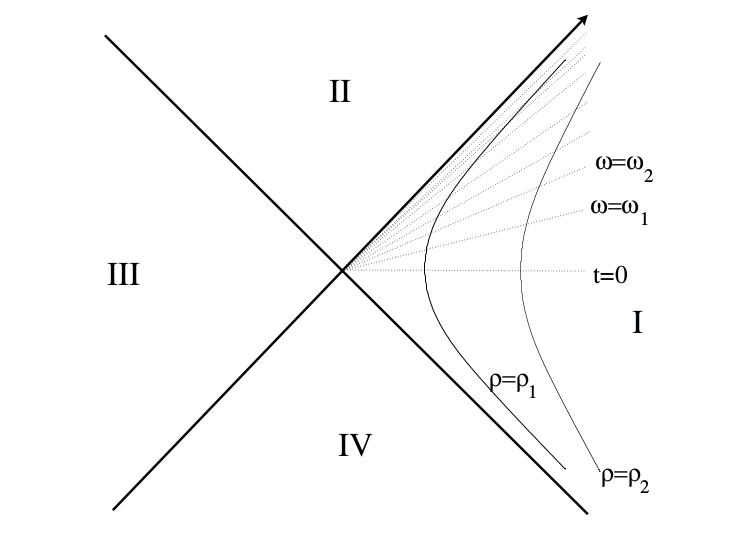
\includegraphics[width=0.8\textwidth]{rindler.png}\hfill
 \caption{Espacio de Minkowski en coordenadas de Rindler (usar imagen libre)
}                   
  \label{fig:rindler}
\end{figure}

Las trayectorias con $\eta=\eta_0$ constante corresponden con observadores que se mueven con
aceleración propia $ae^{-a\xi_0}$.
%\todo{Pq $\xi_0=0$}
El tiempo propio que miden estos observadores es $\tau = e^{a\xi_0}\eta$.
Escogiendo apropiadamente el origen de coordenadas, un observador con aceleración constante
es tiene viene dado por $\eta=\tau$ y $\xi=0$.

Fijándonos en el diagrama de Rindler (figura \ref{fig:rindler}),
un observador con aceleración constante moviéndose a la derecha no puede percibir los 
efectos producidos  en III ni influir en II. 
Además, la información que le llegue de II será percibida como proveniente de un tiempo
infinitamente anterior, por lo que la recta $t=z$ define un horizonte de sucesos futuro y 
la recta $t=-z$ un horizonte de sucesos pasado.

Como el observador acelerado hacia la derecha desconoce el estado del campo en la 
cuña izquierda de Rindler, el estado que percibe no es puro, si no mixto.
La descripción de estados mixtos se realiza mediante una matriz de densidad, que al trazar
sobre los estados desconocidos conduce a que el vacío sea un estado térmico.
Con el fin de hacer la deducción explícita, partimos de la ecuación de Klein-Gordon en
coordenadas de Rindler para la cuña derecha
\begin{equation}
  -\pdv[2]{\phi}{\eta}+\pdv[2]{\phi}{\xi} = 0.
  \label{eq:kgr}
\end{equation}

Definiendo la coordenadas nulas de Rindler 
\begin{equation}
  \begin{gathered}
  u=\eta-\xi,\\
  v=\eta+\xi, 
  \end{gathered}
\end{equation}

la solución general de \ref{eq:kgr} es $\phi(u,v)=\phi_u(u)+\phi_v(v)$, que se expande en los
modos normales
\begin{equation}
  \begin{aligned}
    \phi^u_\omega(u) &=\frac{1}{\sqrt{4\pi\omega}}e^{-i\omega u},\\
    \phi^u_\omega(v) &=\frac{1}{\sqrt{4\pi\omega}}e^{-i\omega v}.
  \end{aligned}
\end{equation}

Aplicaríamos un tratamiento análogo a la cuña izquierda.

El campo propagándose hacia la derecha en coordenadas de Minkowski se expande como
\begin{equation}
  \begin{aligned}
    \phi_U(U)=&\int_0^\infty \Theta(-U)\qty[a^u_\omega \phi^u_\omega(u(U))+a_\omega^{u*}\phi_\omega^u(u(U))^*] \\
    &+\Theta(U)\qty[a^{\tilde u}_\omega \phi^{\tilde u}_\omega(\tilde u(U))+a_\omega^{\tilde u*}\phi_\omega^{\tilde u}(\tilde u(U))^*].
  \end{aligned}
\end{equation}

Donde $\Theta(U)$ es la función de Heaviside 
\begin{equation}
   \Theta(U)=
  \begin{cases}
    0\qquad \text{si }U<0 \\
    1\qquad \text{si }U>0
  \end{cases}
  .
\end{equation}

El cálculo de los coeficientes de Bogoliubov conduce a 
%\todo{Tal vez separar}
\begin{equation}
  \begin{aligned}
    &\alpha_{\omega,\omega'}^{ u} = -\frac{e^{\frac{\pi\omega}{2 a}}}{2\pi a}\sqrt{\frac{\omega}{\omega'}}\qty(\frac{\omega'}{a})^{-i\omega/a}
    \Gamma(i\omega/a), \quad
    \beta_{\omega,\omega'}^{ u} = \frac{e^{-\frac{\pi\omega}{2 a}}}{2\pi a}\sqrt{\frac{\omega}{\omega'}}\qty(\frac{\omega'}{a})^{-i\omega/a}
    \Gamma(i\omega/a)\\
    &\alpha_{\omega,\omega'}^{\tilde u} = -\frac{e^{\frac{\pi\omega}{2 a}}}{2\pi a}\sqrt{\frac{\omega}{\omega'}}\qty(\frac{\omega'}{a})^{i\omega/a}
    \Gamma(-i\omega/a), \quad
    \beta_{\omega,\omega'}^{\tilde u} = \frac{e^{-\frac{\pi\omega}{2 a}}}{2\pi a}\sqrt{\frac{\omega}{\omega'}}\qty(\frac{\omega'}{a})^{i\omega/a} 
    \Gamma(-i\omega/a)
  \end{aligned}
\end{equation}

Por conveniencia, los modos de Unruh se definen como
\begin{equation}
  \begin{aligned}
    \phi^I_\omega(U)=\Theta(-U)\phi^u_\omega(u(U)) + e^{-\frac{\pi\omega}{a}}\Theta(U)\phi_\omega^{\tilde u}(\tilde u(U))^*,\\
    \phi^{II}_\omega(U)=\Theta(U)\phi^{\tilde u}_\omega(\tilde u(U)) + e^{-\frac{\pi\omega}{a}}\Theta(-U)\phi_\omega^{u}(u(U))^*,
  \end{aligned}
\end{equation}
los cuales están definidos en todo el espacio de Minkowski.

La cuantización de los modos de Unruh conduce a los operadores de destrucción
\begin{equation}
  \begin{aligned}
    a_\omega^I = -2\sinh\frac{\pi\omega}{a}\int_0^\infty d\omega' \beta_{\omega\omega'}^{\tilde u} a_{\omega'}^U,\\
    a_\omega^{II} = -2\sinh\frac{\pi\omega}{a}\int_0^\infty d\omega' \beta_{\omega\omega'}^{u} a_{\omega'}^U.\\
  \end{aligned}
\end{equation}

El vacío de estos modos es el vacío de Minkowski, es decir
\begin{equation}
  a_\omega^I \ket{0_H} = a_\omega^{II}\ket{0_H} = 0.
\end{equation}
 
Para buscar el valor esperado de partículas que observa un observador acelerado
en el vacío de Minkowski, primero calculamos
\begin{equation}
  \ev{a_\omega^{u\dagger}a_\omega^u}{0_H} = \int_0^\infty d\omega'' \beta_{\omega\omega''}^u
  \beta_{\omega'\omega''}^{u*} = \frac{1}{e^{\frac{2\pi\omega}{a}}-1}\delta(\omega-\omega').
\end{equation}

En el límite $\omega'\to\omega$, esta cantidad es el valor esperado de partículas que se
detectarían, pero debido a la delta, se obtiene una divergencia.
El motivo es que calcular el número de partículas en toda la cuña derecha de Rindler, 
implica que hay que considerar un observador acelerado eternamente, lo que requiere infinita
energía.
En una situación real, la delta se transformaría en un valor finito.
Por tanto,
\begin{equation}
  \ev{N_\omega^u}{0_H} \sim \frac{1}{e^{\frac{2\pi\omega}{a}}-1}.
\end{equation}

Este valor esperado se corresponde con un sistema de bosones a temperatura $T=a/(2\pi k_B)$.
Sin embargo, todavía no conocemos la forma exacta del vacío de Minkowski.

\todo{Pq usar paquetes? Se puede omitir de la demostración?}
En vez de considerar ondas armónicas con frecuencia bien definida, trabajamos con paquetes
de onda con resolución $\Delta \omega$ centrados en $(n+1/2)\Delta \omega$,
\begin{equation}
  \phi_{n\bar n}^u(u)=\frac{1}{\sqrt{\Delta \omega}}\int_{n\Delta\omega}^{(n+1)\Delta \omega}d\omega e^{i\frac{2\pi \bar n n}{\Delta \omega}\omega}
  \phi^u_\omega(u).
\end{equation}

Al cuantizar estos paquetes se introduce para la cuña derecha el operador destrucción $a_{n\bar n}^u$
y en la cuña izquierda $a_{n\bar n}^{\tilde u}$. 
Construyendo los modos de Unruh asociados a paquetes de ondas, se obtiene que
los operadores que los operadores $a_{n\bar n}^I$ y $a_{n\bar n}^{II}$ cumplen
\begin{equation}
  a_{n\bar n}^I\ket{0_U} = a_{n\bar n}^{II} \ket{0_U} = 0.
\end{equation}

De la expresión de $a_{n\bar n}^I$ y $a_{n\bar n}^{II}$ en términos de $a_{n\bar n}^u$ y $a_{n\bar n}^u$, se llega a 
\begin{equation}
  a_{n\bar n}^{u\dagger} a_{n\bar n}^u \ket{0_U} = a_{n\bar n}^{\tilde u\dagger}a_{n\bar n}^{\tilde u} \ket{0_U},
\end{equation}
y por tanto hay el mismo número de partículas asociadas a paquetes de ondas de Rindler en ambas
cuñas.

Teniendo en cuenta que el estado de vacío ha contener el mismo número de partículas en cada cuña,
\begin{equation}
  \ket{0_H} = \prod_{n,\bar n} \qty(\sum_{m=0}^\infty K_{nm} \ket{m_{n\bar n}}_u\otimes \ket{m_{n\bar n}}_{\bar u}).
\end{equation}
\todo{Es $\prod$ un producto tensorial/ suma directa?}

%\begin{equation}
%  K_{n,m+1}=e^{-\frac{\pi n\Delta \omega }{a}}K_{nm}.
%\end{equation}

%\begin{equation}
%  \ket{0_H} = \prod_{n,\bar n} \qty(\sum_{m=0}^\infty e^{-\frac{\pi n\Delta \omega }{a}}K_{nm}\ket{m_{n\bar n}}_u\otimes \ket{m_{n\bar n}}_{\bar u}).
%\end{equation}

Tras calcular los coeficientes $K_{n \bar n}$ y hacer la traza parcial sobre los estados de
la cuña izquierda, obtenemos que la matriz densidad
\begin{equation}
  \rho  \propto \prod_{n,\bar n} \qty(\sum_{m=0}^\infty e^{-2\pi m n\Delta  \omega/a}\ket{m_{n\bar n}}_u \bra{m_{n\bar n}}_u),
\end{equation}
que describe una distribución de Maxwell-Boltzmann a temperatura $T_U=a/(2\pi k_B)$.
\todo{Contradicción distribución MB vs BE?}

\todo{Omitimos sutilezas de detectores Unruh-DeWitt, cálculo alternativo a la path integral\ldots}

%\begin{equation}
%  \ev{0_U}{N^u_{n,\bar n}} =
%\end{equation}


\section{Radiación de Hawking}
%Introducción relatividad general. Métrica Schwarzschild

El caso más sencillo de agujero negro es el agujero negro de Schwarzschild, que
describe una distribución de masa con simetría esférica y estática. La métrica asociada
es 
\begin{equation}
  ds^2= \qty(1-\frac{2MG}{r})dt^2-\qty(1-\frac{2MG}{r})^{-1}dr^2-r^2d\Omega^2.
\end{equation}

Observamos que en el radio de Schwarzschild $r_s=2MG$, la componente temporal de la 
métrica se anula mientras que la componente radial va a infinito.
Se denomina horizonte de sucesos a la esfera con radio $r_s$ centrada en $r=0$.
%Singularidad


%Coordenadas tortuga

%Transformación de coordenadas. Ecuación de ondas. Modos Boulware.


%Propagación al pasado.




%Para estudiar la física cerca del horizonte es más conveniente emplear las coordenadas
%de Rindler. Para ello sustituimos la coordenada radial por la distancia propia hasta
%el horizonte
%\begin{equation}
%  \rho(r)=\int_0^r dr' \sqrt{g_{rr}(r')}.
%\end{equation}
%
%La métrica se transforma en 
%\begin{equation}
%  ds^2=\qty(1-\frac{2MG}{r(\rho)})dt^2-d\rho^2-r(\rho)^2d\Omega^2.
%\end{equation}
%
%A distancias próximas al horizonte $r\approx r_s$, $\rho\approx 2\sqrt{2MG(r-2MG)}$
%\begin{equation}
%  ds^2\approx \rho^2\qty(\frac{dt}{4MG})^2 -d\rho^2-r(\rho)^2d\Omega^2.
%\end{equation}
%
%Cerca de la coordenada azimutal $\theta=0$, podemos reemplazar las coordenadas
%angulares $\theta,\phi$ por las coordenadas cartesianas $x,y$. Definiendo
%también un tiempo adimensional $\omega=t/(4MG)$ obtenemos la métrica de Rindler
%\begin{equation}
%  ds^2=\rho^2d\omega^2 -d\rho^2 -dx^2-dy^2.
%\end{equation}
%
%Esta métrica describe en realidad un espacio de Minkowski en coordenadas hiperbólicas.
%Si escogemos la transformación
%\begin{align}
%  T&=\rho \sinh \omega, \\
%  Z&=\rho \cosh \omega.
%\end{align}
%la métrica es
%\begin{equation}
%  ds^2=dT^2-dZ^2-dx^2-dy^2.
%\end{equation}
%
%Es conveniente definir un observador fijo para cada punto del espacio, llamado
%FIDO. Estos observadores para mantenerse
%en reposo dentro del campo gravitatorio necesitan una fuerza que los mantenga
%en su sitio. Para los FREFOs, su aceleración es, para $\rho<<MG$ es aproximadamente $1/\rho$.
%
%Si dividimos el espacio de Minkowski en cuatro regiones, el espacio de Rindler ocupa
%la región I. Los FREFOs emplean el las coordenadas del (T,Z,x,y), mientras que
%los FREFOS emplean $(\omega, \rho, x, y)$. El horizonte se sitúa en $T=Z=0$, o
%en coordenadas de Rindler, $\rho=0$.
%Gráficamente, se observa que una translación espacial de $\omega$ para un equivale
%a un boost en el espacio de Minkowski.
%
%Al espacio de Rindler solo le llega información de I y IV, pero la región II está 
%desconectada causalmente por culpa del horizonte.
%Además, un partícula que pase de IV a I será vista como proveniente del tiempo 
%$\omega=-\infty$, por lo que se pueden interpretar como condiciones iniciales.
%
%Estudiamos un campo escalar masivo cuántico $\xi$ en un espacio de Rindler.
%La evolución temporal de un sistema cualquiera viene dada por un hamiltoniano. En el
%espacio de Rindler la evolución en $\omega$ se determina mediante el hamiltoniano de
%Rindler, cuya expresión en función del tensor energía-momento es
%\begin{equation}
%  H_R=\int_0^\infty d\rho dxdy \rho T^{00} (\rho, x, y).
%\end{equation}
%
%En el caso de un campo escalar masivo sometido a un potencial $V$, la densidad de energía
%es
%\begin{equation}
%  T^{00}=\frac{\Pi^2}{2}+\frac{1}{2}\qty(\nabla \xi)^2+V(\xi).
%\end{equation}
%
%Entonces el hamiltoniano es
%\begin{equation}
%  H_R=\int_0^\infty d\rho dx_\perp \frac{\rho}{2}\qty(\Pi^2+\qty(\pdv{\xi}{\rho})^2+\qty(\pdv{\xi}{x_\perp})^2+2V(\xi)).
%\end{equation}
%
%Desde el punto de vista del espacio de Minkowski, $H_R$ es el generador de boosts en 
%la dirección Z.
%
%En una teoría cuántica, el hecho que haya correlación entre el campo para dos puntos
%del espacio origina un fenómeno interesante en el espacio de Rindler. 
%Hemos visto que la región III está desconectada de la región I, por lo que consideramos
%al campo en cada región como subsistemas distintos. Pero debido a que el campo en I está
%correlacionado con el campo III, están entrelazados entre sí.
%Por esta razón, no podemos describir al campo en I como un sistema puro como una
%matriz de densidad obtenida tomando la traza parcial en III de la matriz de densidad
%del sistema completo.
%
%En general, si el estado asociado a dos subsistemas A y B que no están interactuando 
%es $\ket{\Psi}$, su matriz de densidad es
%\begin{equation}
%  \rho_{AB}=\ket{\Psi}\bra{\Psi}.
%\end{equation}
%
%La matriz de densidad que describe el sistema A es
%\begin{equation}
%  \rho_{A}=\Tr_B \rho_{AB}=\expval{\rho_{AB}}{\beta}.
%\end{equation}
% 
%A cada matriz de densidad le corresponde la entropía de von Neumann
%\begin{equation}
%  S=-\Tr (\rho_A \ln \rho_A)=-\sum_j \rho_j \ln \rho_j.
%\end{equation}
%
%Donde $\rho_j$ son los valores propios de $\rho_A$.
%Esta entropía se debe a que estamos perdiendo información al ignorar el subsistema $B$, que 
%está entrelazado con $A$, por lo que también se denomina entropía de entrelazamiento.
%La interpretación de $\rho_j$ es que estamos describiendo un sistema cuyo estado no 
%conocemos, pero sabemos que a cada estado le corresponde una probabilidad $\rho_j$.
%
%Por otro lado un sistema termodinámico en equilibrio a temperatura $\beta$ tiene 
%asociado la matriz densidad 
%\begin{equation}
%  \rho=\frac{e^{-\beta H}}{\Tr e^{\beta H}}.
%\end{equation}
%
%Retomamos el campo escalar en un espacio de Rindler. 
%Para $T=0$, los campos en cada punto forman un conjunto completo de observables que 
%conmutan. Denominamos $\xi_L$ a los campos en $Z<0$ y $\xi_R$ si $Z>0$.
%En teoría cuántica de campos, un estado se describe como una distribución que 
%depende de los campos $\Psi[\xi]=\Psi[\xi_L,\xi_R]$.
%
%Supondremos que $\Psi[\xi_L,\xi_R]$ está en el estado fundamental (vacío) del hamiltoniano
%de Minkowski. Para hallar el estado fundamental mediante la integral de camino 
%en mecánica cuántica de partículas aplicamos
%\begin{align}
%  \braket{y,T}{x,0}\sim \int_{X(0)=x,X(T)=y} \mathcal D X e^{-S} \sim 
%  \mel{y}{e^{-HT}}{x}=\sum_{n,n'} \ip{y}{n}\mel{n}{e^{-HT}}{n'}\ip{n'}{n}=\\
%  =\sum_{n,n'} \Psi_n(y) e^{-E_n T} \bar{\Psi}_n(x)\sim   \Psi_0(y) e^{-E_0 T} \bar{\Psi}_0(x).
%\end{align}
%
%Donde hemos aplicado una rotación de Wick $t\to T=it$ por continuación analítica.
%Por lo que $\bar{\Psi}_0(x)\sim \int_{X(0)=x} \mathcal D x e^{-S}$.
%De forma similar en teoría cuántica de campos 
%\begin{equation}
%  \Psi[\xi_L,\xi_R]=\frac{1}{\sqrt{Z}}\int_{X^0>0, \xi(X^0=0)=(\xi_L,\xi_R)} e^{-S}
%\end{equation}
%
%Para evaluar la integral, tenemos en cuenta que como la translación en $\omega$
%equivale a un boost en el espacio de Minkowski, en el espacio euclídeo se traduce
%en una rotación.
%El ángulo $\theta$ con respecto al eje $Z$ en el plano $(Z,X^0)$ se corresponde con
%el tiempo de Rindler $\omega$.


\chapter{Cuerdas en espacios curvos}


\chapter{Conclusión}


%\nocite{*}
\bibliographystyle{babunsrt}
\bibliography{mybib}
\end{document}
